\section{Model}

\subsection{Experimental Design}
\begin{figure}[h]
    	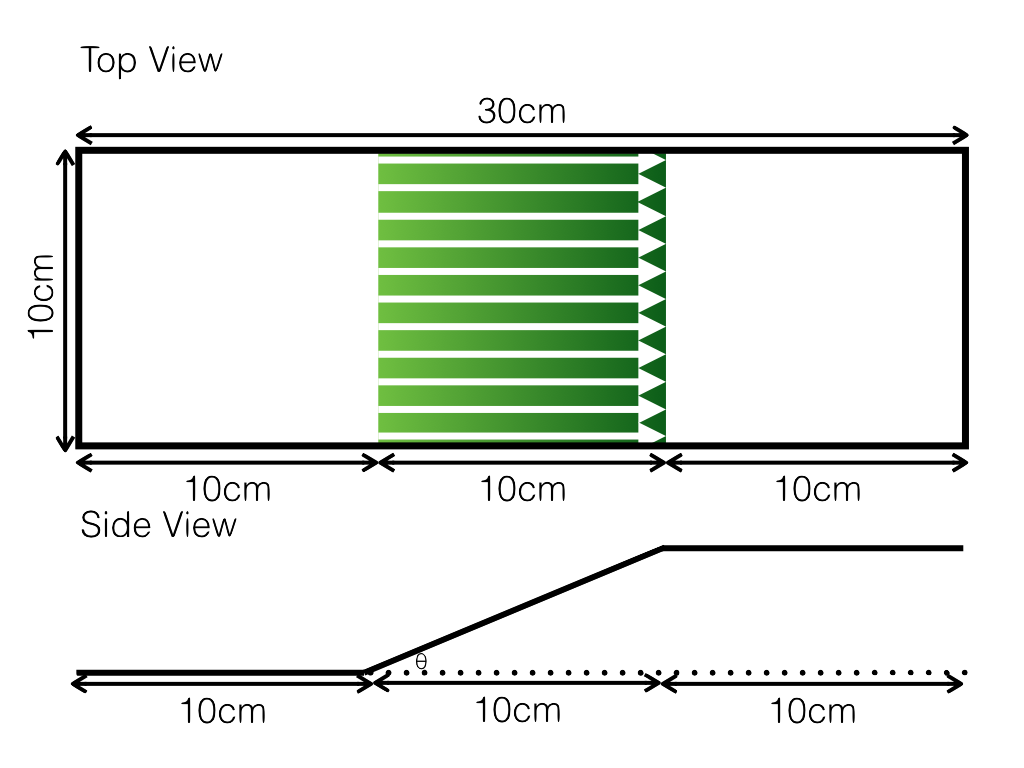
\includegraphics[width=0.4\textwidth]{img/model_components_cartoons_011}
      \caption{Arena terrain scheme}
\end{figure}






\begin{figure}[h]
    	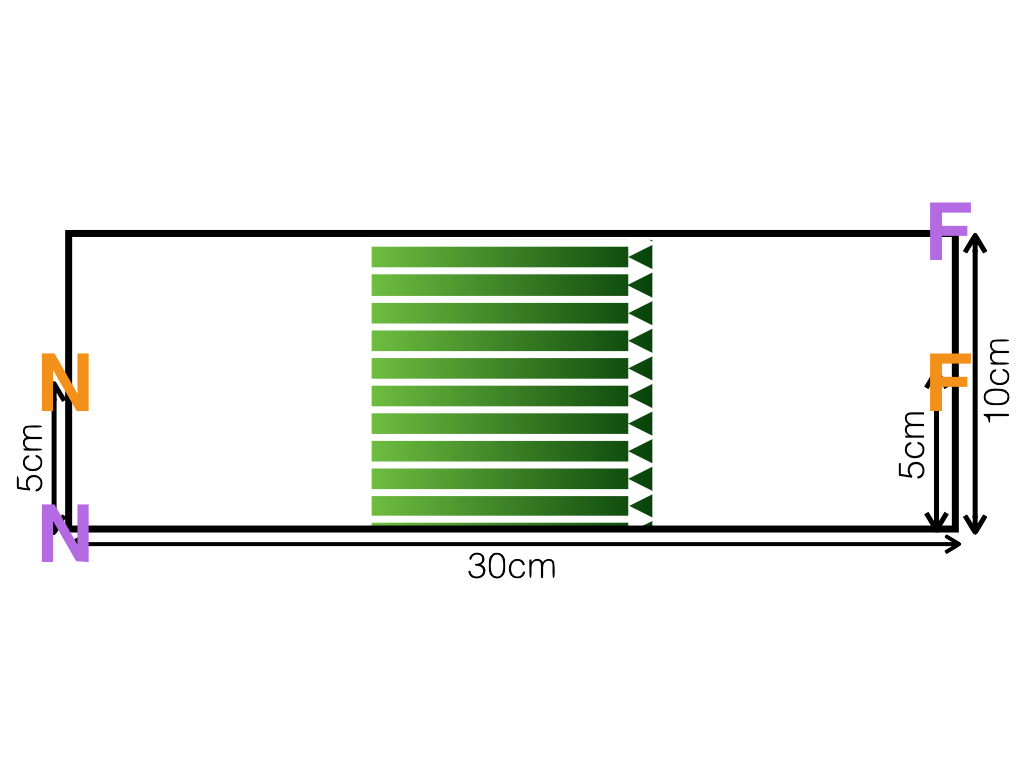
\includegraphics[width=0.4\textwidth]{img/model_components_cartoons_010}
				\vspace{-8ex}
				\caption{Nest and food placement scheme}
\end{figure}


\subsection{Modeling Considerations}

The model should consider:
	\begin{itemize}
    	\item self-propulsion,
        \item containment in arena,
        \item forager/returner roles (attraction to food, attraction to nest),
        \item random reorientation events (``Boltzmann walker''),
        \item physical effects of gravity on inclined terrain,
        \item behavioral phenomena on inclined terrain,
        \item pheromone deposit, and
        \item pheromone response behavior.
    \end{itemize}


\subsection{Random Reorientation Events (''Boltzmann Walker'')}
\begin{figure}[h]	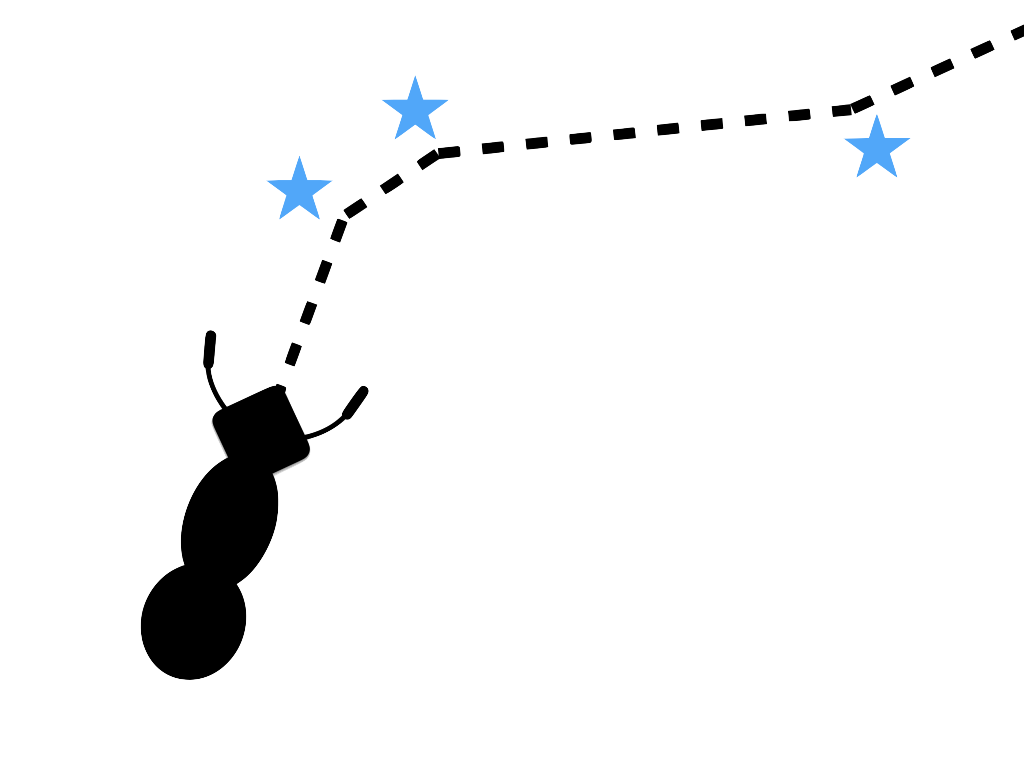
\includegraphics[width=0.4\textwidth]{img/model_components_cartoons_009}
		\caption{\footnotesize{``Boltzmann walker'' cartoon; blue stars denote random reorientation events.}}
\end{figure}
\begin{align*}
\frac{d}{dt} \begin{pmatrix}\vec{x}\\\vec{v}\\s\end{pmatrix} = \begin{pmatrix}\ldots \\ \ldots\\ \norm{v}\end{pmatrix}
\end{align*}
\begin{align*}
\theta_{\operatorname{new}} = \theta_{\operatorname{old}} + \bm{T} \\
s = 0 \\
s_{\operatorname{thresh}} = \bm{X}
\end{align*}


\begin{itemize}
		\item ant ``keeps track'' of how far it has traveled, $s$
    \item upon reaching a threshold distance ($s > s_{\operatorname{thresh}}$), the ant experiences a ``reorientation event''
    \item the threshold distance is generated from an exponential distribution ($\bm{X} \sim \mathit{exp}(\omega)$)
    \item ``memoryless property'' (probability of reorientation is uniform over every unit of distance the ant traverses)
    \item the angle the ant turns through is normally distributed  ($\Delta \theta = \bm{T} \sim \mathcal{N}(0,\sigma^2)$)
\end{itemize}

\subsection{Random Reorientation Events (``Boltzmann Walker'')}
\begin{align*}
\bm{T}_{\operatorname{effective}} = \bm{T} / \beta \\
\beta =
\begin{cases}
      \text{forager role} & e^{c_1p} \\
      \text{returner role} & c_2
\end{cases} \\
s_{\operatorname{thresh}} = \bm{X} + c_3 \frac{|\vec{s} \cdot \vec{v}|}{\norm{\vec{v}}}
\end{align*}

\begin{itemize}
  \item free path of ant ($s_{\operatorname{thresh}}$) increases if ant oriented with the gradient {\scriptsize\cite{khuong_how_2013}}
	\item severity of random reorientation should decrease with
    \begin{itemize}
    	\item pheromone detection (``following trail'')
      \item returner status
    \end{itemize}
    \item $p$ is maximum pheromone level sensed by ant
\end{itemize}

\subsection{Behavioral Response to Incline}

\begin{figure}[h]
\begin{minipage}[]{0.3\textwidth}
    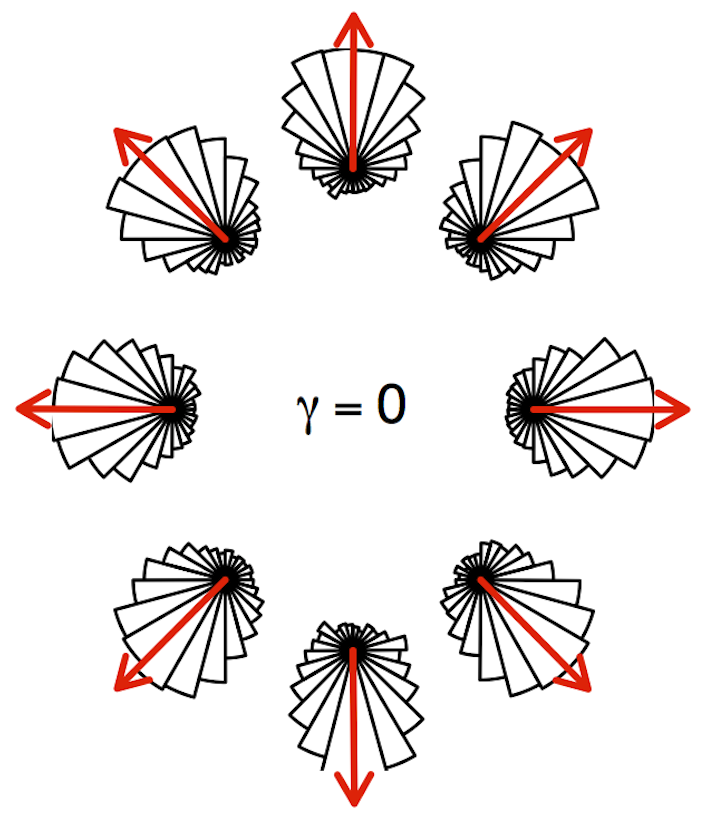
\includegraphics[width=\textwidth]{img/khuong_0}
\end{minipage}%
\begin{minipage}[]{0.05\textwidth}
~
\end{minipage}%
\begin{minipage}[]{0.3\textwidth}
    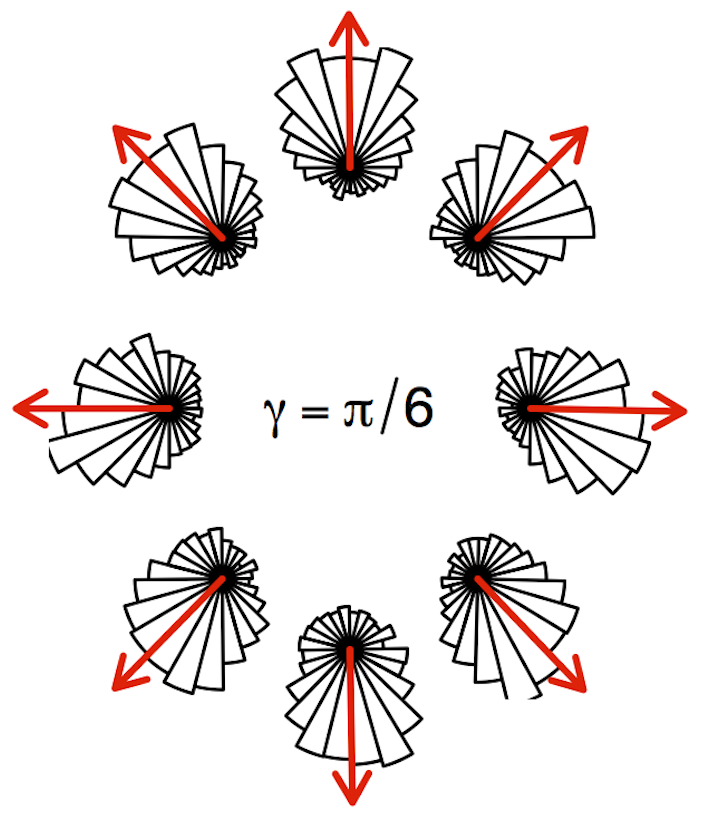
\includegraphics[width=\textwidth]{img/khuong_pi_div_6}
\end{minipage}%
\begin{minipage}[]{0.05\textwidth}
~
\end{minipage}%
\begin{minipage}[]{0.3\textwidth}
    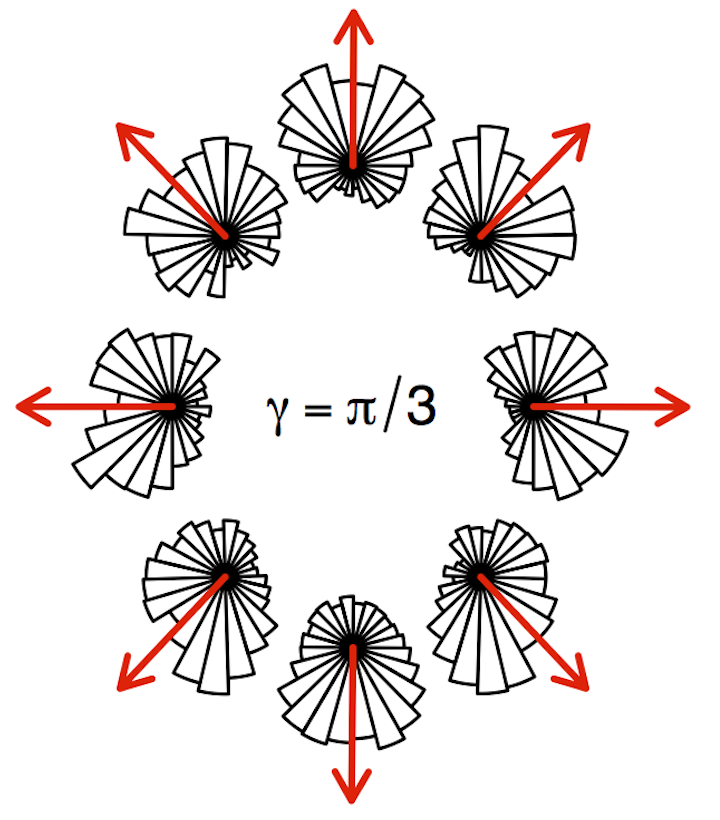
\includegraphics[width=\textwidth]{img/khuong_pi_div_3}
\end{minipage}%
\caption{Ant Reorientation on Inclined Surfaces \scriptsize{\cite{khuong_how_2013}}}
\end{figure}


\begin{itemize}
	\item ants preferentially re-orient themselves to align with or against a surface's topographical gradient {\cite{khuong_how_2013}}
    \item ants follow longer free paths when aligned with or against a surface's topographical gradient {\scriptsize\cite{khuong_how_2013}}
\end{itemize}


\subsection{Response to Pheromone}
\begin{align*}
\frac{d}{dt} \begin{pmatrix}\vec{x}\\\vec{v}\end{pmatrix} = \begin{pmatrix}\hdots\\ \hat{\vec{v}}_{\perp}(L - R)\end{pmatrix}
\end{align*}
\begin{itemize}
	\item ant integrates pheromone concentration over ``L'' and ``R'' quarter-circular regions
    \item ant accelerates perpendicular to its orientation
    \item magnitude of acceleration is proportional to the difference in concentration of pheromone over the ``L'' and ``R'' regions
\end{itemize}


\subsection{Self Propulsion}

\begin{align*}
			\frac{d}{dt} \begin{pmatrix}\vec{x}\\\vec{v}\end{pmatrix} = \begin{pmatrix}\vec{v}\\ \alpha \hat{\vec{v}}(\xi^2 - \norm{\vec{v}}^2)\end{pmatrix}
\end{align*}

\begin{itemize}
	\item ant accelerates in the direction of its movement if $\norm{\vec{v}}  \xi$
    \item ant accelerates against the direction of its movement if $\norm{\vec{v}} < \xi$
    \item``pushes'' ant towards a fixed speed
    \item $\alpha$ is a constant that governs the magnitude of this effect
\end{itemize}

\subsection{Attraction to Food/Nest}
\begin{align*}
\frac{d}{dt} \begin{pmatrix}\vec{x}\\\vec{v}\end{pmatrix} = \begin{pmatrix}\hdots \\ \beta_{\vec{x}} \frac{\vec{a} - \vec{x}}{\norm{\vec{a} - \vec{x}}} \end{pmatrix}
\end{align*}
\begin{itemize}
	\item ant experiences nest attraction if it is in the returner role
    \item ant experiences food attraction if it is in the forager role
	\item ant accelerates in the direction of the attractor
    \item if multiple attractors are present,
    \begin{itemize}
		\item ant is attracted to nearest food item
        \item ant is attracted to midpoint of nest items
    \end{itemize}
    \item $\beta_{\vec{x}}$ governs the strength of attraction
    \begin{itemize}
    	\item constant for nest attraction
        \item for food attraction, decays exponentially with distance from food
    \end{itemize}
\end{itemize}

\subsection{Near Nest Attraction}
\begin{align*}
\frac{d}{dt} \begin{pmatrix}\vec{x}\\\vec{v}\end{pmatrix} = \begin{pmatrix}
\hdots \\
\gamma_{\vec{x}} \hat{\vec{v}}_{\perp} \Big( \hat{\vec{v}}_{\perp} \cdot \frac{\vec{a} - \vec{x}}{\norm{\vec{a} - \vec{x}}} \Big)
\end{pmatrix}  \\
\beta = c_1e^{-c_2\norm{\vec{a} - \vec{x}}}
\end{align*}
\begin{itemize}
	\item ant experiences attraction with magnitude increasing exponentially with proximity to nest
    \item acceleration is projected onto vector perpendicular to orientation of ant
	\item ensures that ant goes directly to nest if ant is nearby the nest
\end{itemize}

\subsection{Pheromone Deposit}
\begin{align*}
\frac{d}{dt} p = \kappa f(p,s\vec{x}_1,\hdots,\vec{x}_n)
\end{align*}
\begin{itemize}
	\item the rate of pheromone deposit is proportional to total speed of ants located at a tile
    \item (ants only deposit pheromone when they move)
    \item let $f(p, \vec{x}_1,\hdots,\vec{x}_n)$ represent a sum of the speeds of of ants associated with the pheromone point $p$
    \item $\kappa$ is a constant governing the magnitude of pheromone deposit
\end{itemize}

\subsection{Complete Model}

\scriptsize
\centerline{
\begin{minipage}{\linewidth}
\begin{align*}
\frac{d}{dt}
\begin{pmatrix}
    \vec{x}_1 \\
    \vec{v}_1 \\
    s_1 \\
    \vdots \\
    p_1 \\
    \vdots
\end{pmatrix}
= \begin{pmatrix}
	\vec{v}_1 \\
    \alpha \hat{\vec{v}}_1 \Big[ \frac{c}{\norm{\vec{v}}} - a \norm{\vec{v}} + \frac{\norm{\vec{v}}^2 - b \vec{v} \cdot \nabla s}{\sqrt{\norm{\vec{v}}^2 + (\vec{v} \cdot \nabla s)^2}} \Big] + \beta_{\vec{x}} \frac{\vec{a} - \vec{x}_1}{\norm{\vec{a} - \vec{x}_1}} + \hat{\vec{v}}_{1\perp}(L_1 - R_1) + \gamma_{\vec{x}} \hat{\vec{v}}_{\perp} \Big( \hat{\vec{v}}_{\perp} \cdot \frac{\vec{a} - \vec{x}}{\norm{\vec{a} - \vec{x}}} \Big) \\
    \norm{\vec{v}_1} \\
    \vdots \\
    \kappa f(p_1, \vec{x}_1,\hdots,\vec{x}_n) + \lambda p_1 \\
    \vdots
\end{pmatrix}
\end{align*}
\end{minipage}
}
\normalsize
events:
\begin{itemize}
\item out of bounds $\rightarrow$ reflect heading to ``bounce'' ant
\item $s > s_{\operatorname{thresh}}$ $\rightarrow$ $s = 0$, $s_{\operatorname{thresh}} = \bm{X} + c_3 \frac{|\vec{s} \cdot \vec{v}|}{\norm{\vec{v}}}$, random reorientation event with gradient alignment bias
\item close to food/nest $\rightarrow$ switch forager/returner role
\end{itemize}

\subsection{Table of Parameters}
\noindent
\pgfplotstabletypeset[
    begin table=\begin{longtable},
    end table=\end{longtable}, 
    string type,
    col sep=comma,
    columns={name,value,unit,notes},
    columns/name/.style={column type=l},
    columns/value/.style={column type=c},
    columns/unit/.style={column type=c},
    columns/notes/.style={column type=P},
    every head row/.style={
        before row=\toprule,
        after row=
            \cmidrule(lr){1-1}
            \cmidrule(lr){2-2}
            \cmidrule(lr){3-3}
            \cmidrule(lr){4-4}
    },
    every last row/.style={after row=\bottomrule}
    ]{consts.csv}
